%15 min preso!
\documentclass[xcolor=table,aspectratio=169]{beamer}
\usepackage{beamerthemesplit}
\usepackage{wrapfig}
\usetheme{SPbGU}
\usepackage{pdfpages}
\usepackage{amsmath}
\usepackage{cmap}
\usepackage[T2A]{fontenc}
\usepackage[utf8]{inputenc}
\usepackage[english]{babel}
\usepackage{indentfirst}
\usepackage{amsmath}
\usepackage{tikz}
\usepackage{multirow}
\usepackage[noend]{algpseudocode}
\usepackage{algorithm}
\usepackage{algorithmicx}
\usepackage{fancyvrb}
\usepackage{hyperref} 
\usetikzlibrary{calc}
\usetikzlibrary{shapes, backgrounds}
\usetikzlibrary{arrows,automata}
\usetikzlibrary{positioning}
\usetikzlibrary{fit}
\usetikzlibrary{shapes.callouts}
\usetikzlibrary{shapes.misc}
\usepackage{xparse}
\usepackage{fontawesome}

\usepackage{etoolbox,refcount}
\usepackage{multicol}

\usepackage{tabularx}
\newcolumntype{Y}{>{\raggedleft\arraybackslash}X}

\renewcommand{\thealgorithm}{}

\newtheorem{mytheorem}{Theorem}
\renewcommand{\thealgorithm}{}

\newcommand{\tikzmark}[1]{\tikz[overlay,remember picture] \node (#1) {};}
\def\Put(#1,#2)#3{\leavevmode\makebox(0,0){\put(#1,#2){#3}}}

\newcommand{\ltz}{$< 1$}

\tikzset{
    state/.style={
           rectangle,
           rounded corners,
           draw=black, very thick,
           minimum height=2em,
           inner sep=2pt,
           text centered,
           },
}

\tikzset{
    invisible/.style={opacity=0,text opacity=0},
    visible on/.style={alt=#1{}{invisible}},
    alt/.code args={<#1>#2#3}{%
      \alt<#1>{\pgfkeysalso{#2}}{\pgfkeysalso{#3}} % \pgfkeysalso doesn't change the path
    },
}

\tikzset{cross/.style={cross out, draw=black, minimum size=2*(#1-\pgflinewidth), inner sep=0pt, outer sep=0pt, ultra thick},
%default radius will be 1pt. 
cross/.default={1pt}}

\NewDocumentCommand{\mycallout}{r<> O{opacity=0.8,text opacity=1} m m m}{%
\tikz[remember picture, overlay]\node[align=center, fill=cyan!20, text width=#5cm,
#2,visible on=<#1>, rounded corners,
draw,rectangle callout,anchor=pointer,callout relative pointer={(290:0.5cm)}]
at (#3) {#4};
}

\NewDocumentCommand{\mycalloutR}{r<> O{opacity=0.8,text opacity=1} m m m}{%
\tikz[remember picture, overlay]\node[align=center, fill=cyan!20, text width=#5cm,
#2,visible on=<#1>, rounded corners,
draw,rectangle callout,anchor=pointer,callout relative pointer={(30:0.8cm)}]
at (#3) {#4};
}


%callout relative pointer={(230:0.5cm)}]
\setbeamertemplate{page number in head/foot}[appendixframenumber]
\newcounter{countitems}
\newcounter{nextitemizecount}
\newcommand{\setupcountitems}{%
  \stepcounter{nextitemizecount}%
  \setcounter{countitems}{0}%
  \preto\item{\stepcounter{countitems}}%
}
\makeatletter
\newcommand{\computecountitems}{%
  \edef\@currentlabel{\number\c@countitems}%
  \label{countitems@\number\numexpr\value{nextitemizecount}-1\relax}%
}
\newcommand{\nextitemizecount}{%
  \getrefnumber{countitems@\number\c@nextitemizecount}%
}
\newcommand{\previtemizecount}{%
  \getrefnumber{countitems@\number\numexpr\value{nextitemizecount}-1\relax}%
}
\makeatother    
\newenvironment{AutoMultiColItemize}{%
\ifnumcomp{\nextitemizecount}{>}{3}{\begin{multicols}{2}}{}%
\setupcountitems\begin{itemize}}%
{\end{itemize}%
\unskip\computecountitems\ifnumcomp{\previtemizecount}{>}{3}{\end{multicols}}{}}

\definecolor{links}{HTML}{2A1B81}
\hypersetup{colorlinks,linkcolor=,urlcolor=links}


\newcommand\colR{\cellcolor{red!20}}
\newcommand\colB{\cellcolor{blue!20}}
\newcommand\colG{\cellcolor{green!20}}

\beamertemplatenavigationsymbolsempty

\title[GPGPU и RISC-V]{Вычисления на графических ускорителях в экосистеме RISC-V}
\institute[СПбГУ]{
Санкт-Петербургский Государственный Университет
}

% То, что в квадратных скобках, отображается в левом нижнем углу.
\author[Семён Григорьев]{\textbf{\underline{Семён Григорьев}} \\Полина Угарова, Екатерина Арзамасцева, Даниил Правкин, Шамиль Шаехмитов, Владимир Кутуев}

\date{29 сентября 2026г.}

\begin{document}
{
\begin{frame}[fragile]
  \begin{table}
  \centering
  \begin{tabularx}{\linewidth}{XcX}
    
\includegraphics[height=1.4cm]{pictures/RuSCDays_logo_blue.pdf} \hfill
    & 
    & \hfill 
\includegraphics[height=1.6cm]{pictures/SPbGU_Logo.png}
  \end{tabularx}
  \end{table}
  \titlepage
\end{frame}
}

\begin{frame}[fragile]
  \frametitle{Контекст: вычисления, а не графика}
  \begin{itemize}
    \item \textbf{Spla\footnote{\url{https://github.com/SparseLinearAlgebra/spla}}}: \emph{алгоритмы анализа графов на основе разреженной обобщённой линейной алгебры}, реализация подмножества GraphBLAS\footnote{\url{https://graphblas.org/}}-подобного API на C++ и OpenCL C
    \begin{itemize}
      \item Переносимое решение между GPGPU разных вендоров
      \item Запускается на CPU благодаря POCL
      \item На <<взрослых>> GPGPU конкурентно с аналогами
      \item Неплохой тест на <<зрелость>> поддержки OpenCL на устройстве
    \end{itemize}
    \pause
    \item  \textbf{CLBlast}\footnote{\url{https://github.com/CNugteren/CLBlast}}: вычислительная линейная алгебра (плотная)
    \begin{itemize}
      \item Переносимое решение между GPGPU разных вендоров (за счёт OpenCL)
      \item Оптимизированные, в том числе под мобильные GPGPU, ядра
      \item Неплохой тест на поддержку классических оптимизаций
    \end{itemize}
  \end{itemize}
  \pause
  \begin{center}
    \textbf{Работоспособность, не анализ производительности}
  \end{center}
\end{frame}

\begin{frame}[fragile]
  \frametitle{RISC-V и GPGPU}
  \begin{itemize}
    \item \textbf{RISC-V CPU + Imagination Technologies GPU}: самая распространённая (из доступных) конфигурация
    \pause
    \item \textbf{RISC-V CPU + AMD GPU}: работает и есть официальная поддержка (\href{https://milkv.io/pioneer}{Milk-V Pioneer}, \href{https://riscv.org/ecosystem-news/2024/10/risc-v-cpu-demoed-with-rx-7900-xtx-gpu-in-debian-linux-amd-flagship-gpu-paired-with-milk-v-megrez-board-and-sifive-p550-cores/}{Milk-V Megrez}, \href{https://milkv.io/ruyibook}{RuyiBook})
    \item \textbf{RISC-V CPU + Intel GPU}: \href{https://www.reddit.com/r/RISCV/comments/1ftep9u/intel_arc_a770_on_riscv/}{ходят слухи, что можно}, но официальной поддержки пока нет
    \item \textbf{RISC-V CPU + Nvidia GPU}: \href{https://riscv.org/ecosystem-news/2025/07/nvidia-to-bring-cuda-platform-support-to-the-risc-v/}{анонсировано}
    \pause
    \item \textbf{RISC-V GPU} (открытые проекты с полным стеком)
    \begin{itemize}
      \item \href{https://github.com/vortexgpgpu/vortex}{Vortex}
      \item \href{https://github.com/THU-DSP-LAB/ventus-gpgpu}{Ventus}
    \end{itemize}
  \end{itemize}
\end{frame}

\begin{frame}
  \frametitle{RISC-V CPU + Imagination Technologies GPU: SpacemiT M1 (RISC-V) с IMG BXE-2-32 GPU}
\begin{itemize}
  \item OpenCL
  \item POCL
  \item Есть проблемы и тонкости
  \begin{itemize}
    \item !!!
    \item !!!
  \end{itemize}
\end{itemize}
\end{frame}

\begin{frame}
  \frametitle{\textbf{Spla} на SpacemiT M1 (RISC-V) с IMG BXE-2-32 GPU}
\begin{columns}
        \column{0.5\textwidth}        
        \vspace{-0.5cm}
        \begin{center}
          BFS \\
        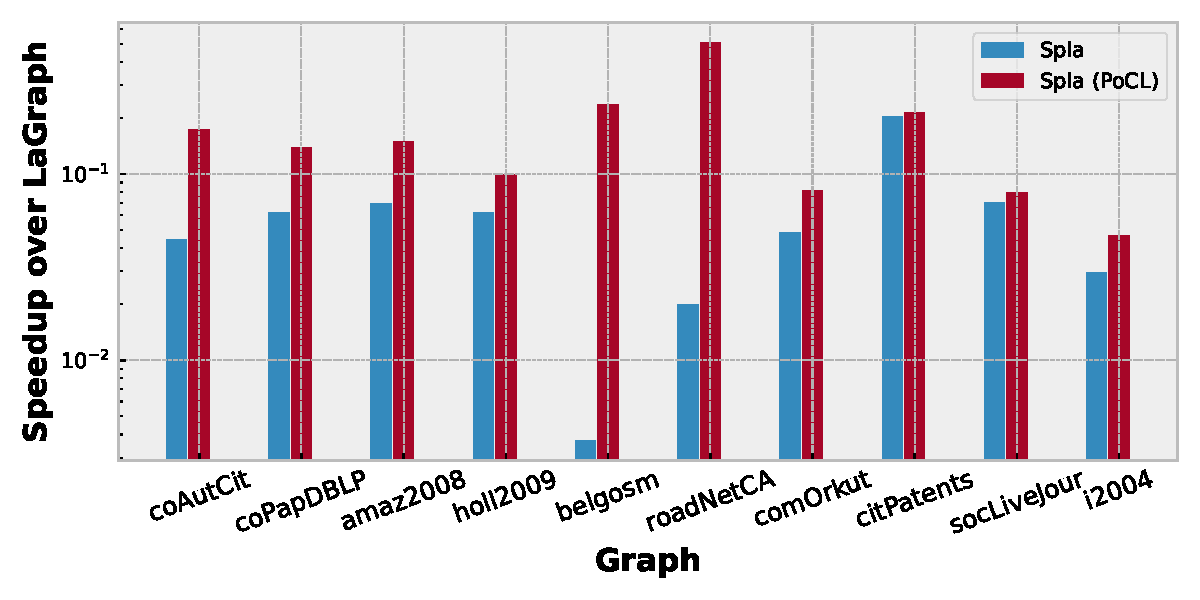
\includegraphics[width=0.909\linewidth]{pictures/rq1_rel_bfs.pdf}
        Single Source Shortest Path \\
        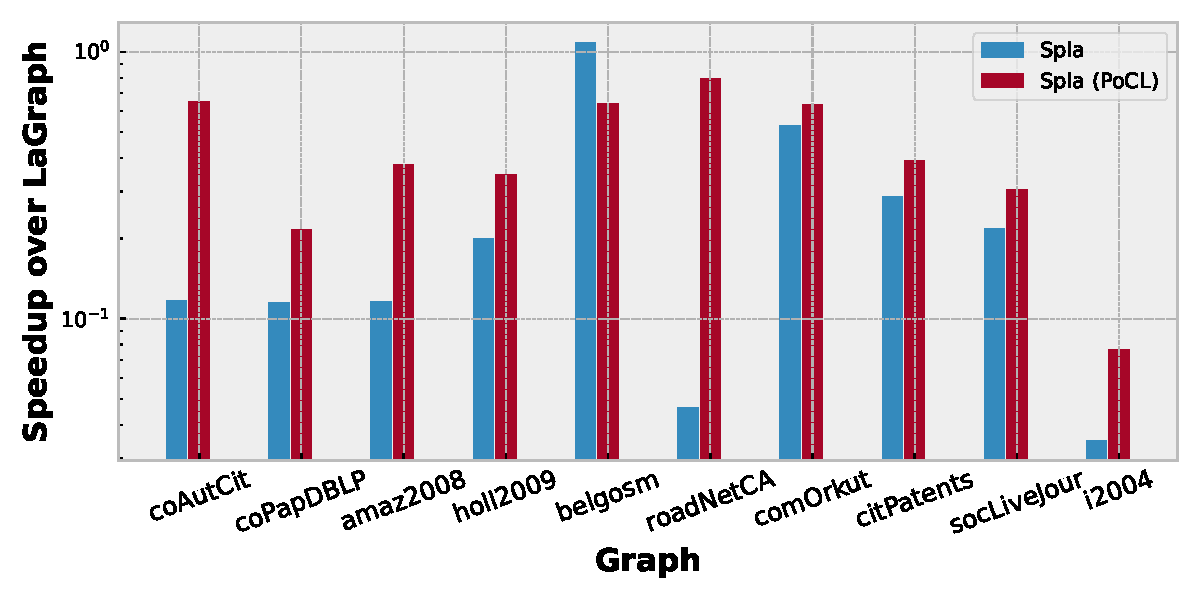
\includegraphics[width=0.909\linewidth]{pictures/rq1_rel_sssp.pdf}
        \end{center}
        \column{0.5\textwidth}
        \vspace{-0.5cm}
        \begin{center}
          Triangle Count\\
        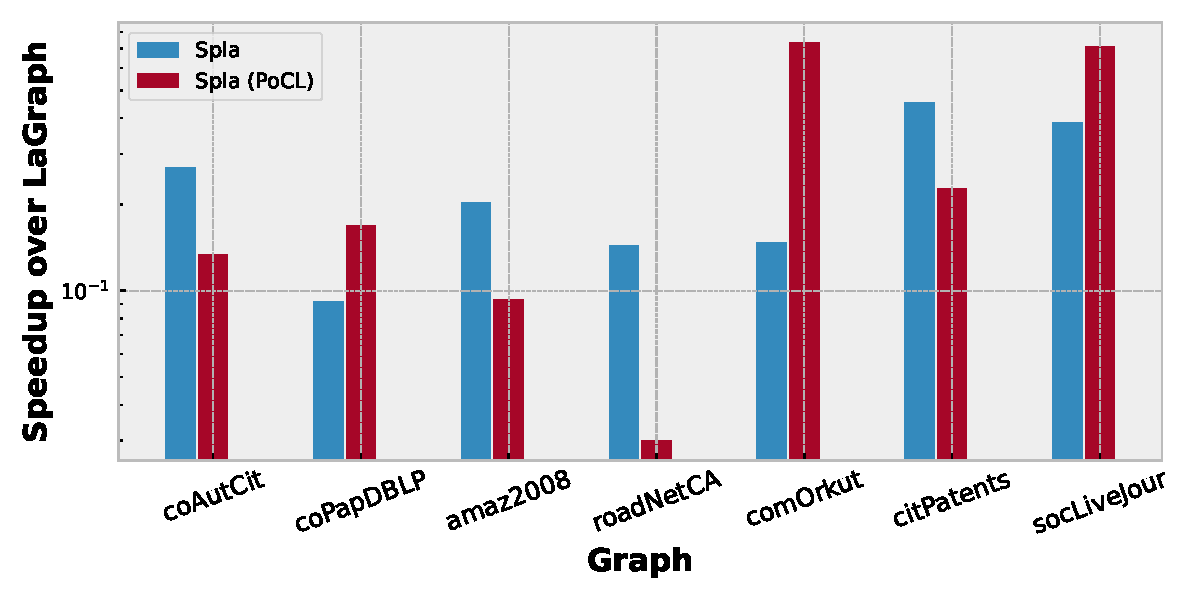
\includegraphics[width=0.9\linewidth]{pictures/rq1_rel_tc.pdf}
        PageRank\\
        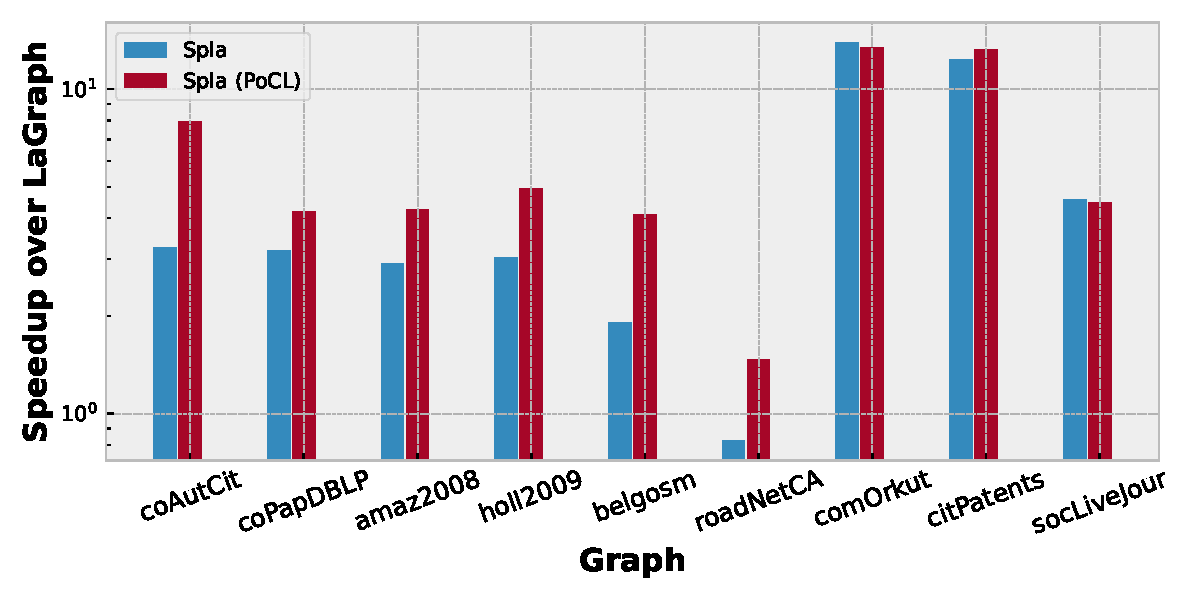
\includegraphics[width=0.9\linewidth]{pictures/rq1_rel_pr.pdf}
        \end{center}
    \end{columns}
    
\end{frame}

\begin{frame}
  \frametitle{Результаты умножения плотных матриц на SpacemiT M1 с IMG GPU}
  \begin{center}
  \tikzmark{z1}{ }
  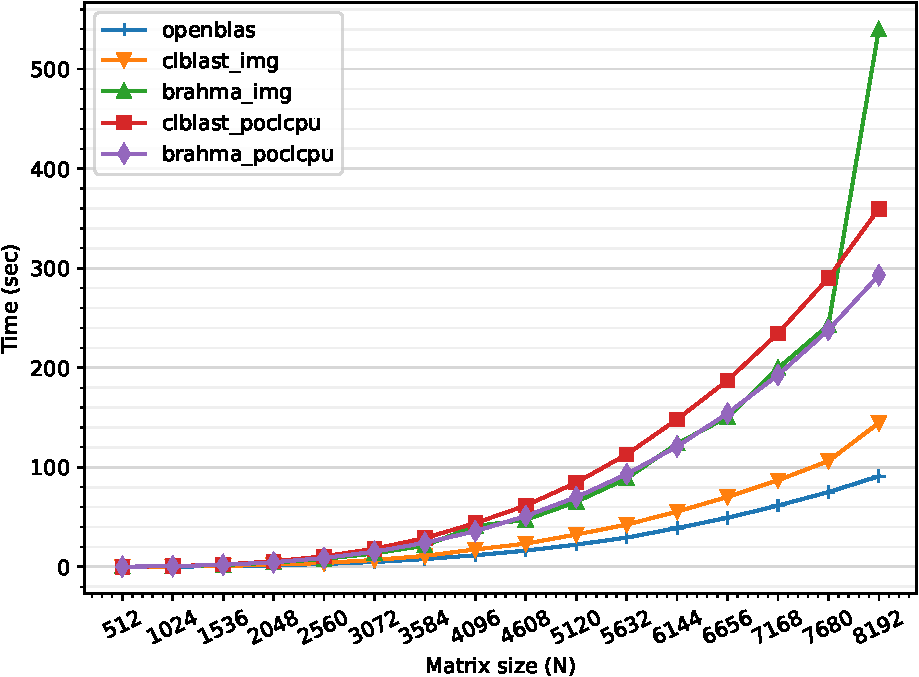
\includegraphics[width=0.55\textwidth]{pictures/MILK-V_crop.pdf}
  \tikz[overlay,remember picture]{\draw[draw=red,thick,double,fill opacity=0.2] ($ (z1) + (1.1,5.45)$) rectangle ($ (z1) + (3.4,6.05)$);}
  \\
    (Некоторые) GPGPU от Imagination Technologies (пока) не совсем для вычислений
  \end{center}
\end{frame}

\begin{frame}[fragile]
  \frametitle{Запуск <<дискретных>> GPGPU на Milk-V (SpacemiT M1)}
  \begin{itemize}
    \item[\faCheck] Старый AMD (Radeon HD 6450)
    \begin{itemize}
      \item Запускается <<из коробки>>
      \item Работают прикладные алгоритмы на основе Spla
    \end{itemize} 
    \item[\faGears] Должно быть возможно, но нужно конфигурировать и собирать ядро
    \begin{itemize} 
      \item Новый AMD (RX 6750) 
        \begin{itemize}
          \item Работа идёт: \url{https://www.phoronix.com/news/AMDKFD-RISC-V-Linux-6.16}
          \item Команда Yadro смогла подключить AMD GPGPU к RISC-V ядру на ПЛИС: \url{https://habr.com/ru/companies/yadro/articles/946950/}
        \end{itemize} 
      \item Intel ARC
        \begin{itemize}
          \item Работа идёт:  \url{https://habr.com/ru/companies/selectel/articles/966828/}          
        \end{itemize}
      \item Nvidia, скорее всего, через \href{https://nouveau.freedesktop.org/}{nouveau} \textit{[nuvo]}
    \end{itemize}
  \end{itemize}
\end{frame}

\begin{frame}
  \frametitle{Boruvka MST на  Milk-V + AMD Radeon HD 6450}
        \begin{center}
        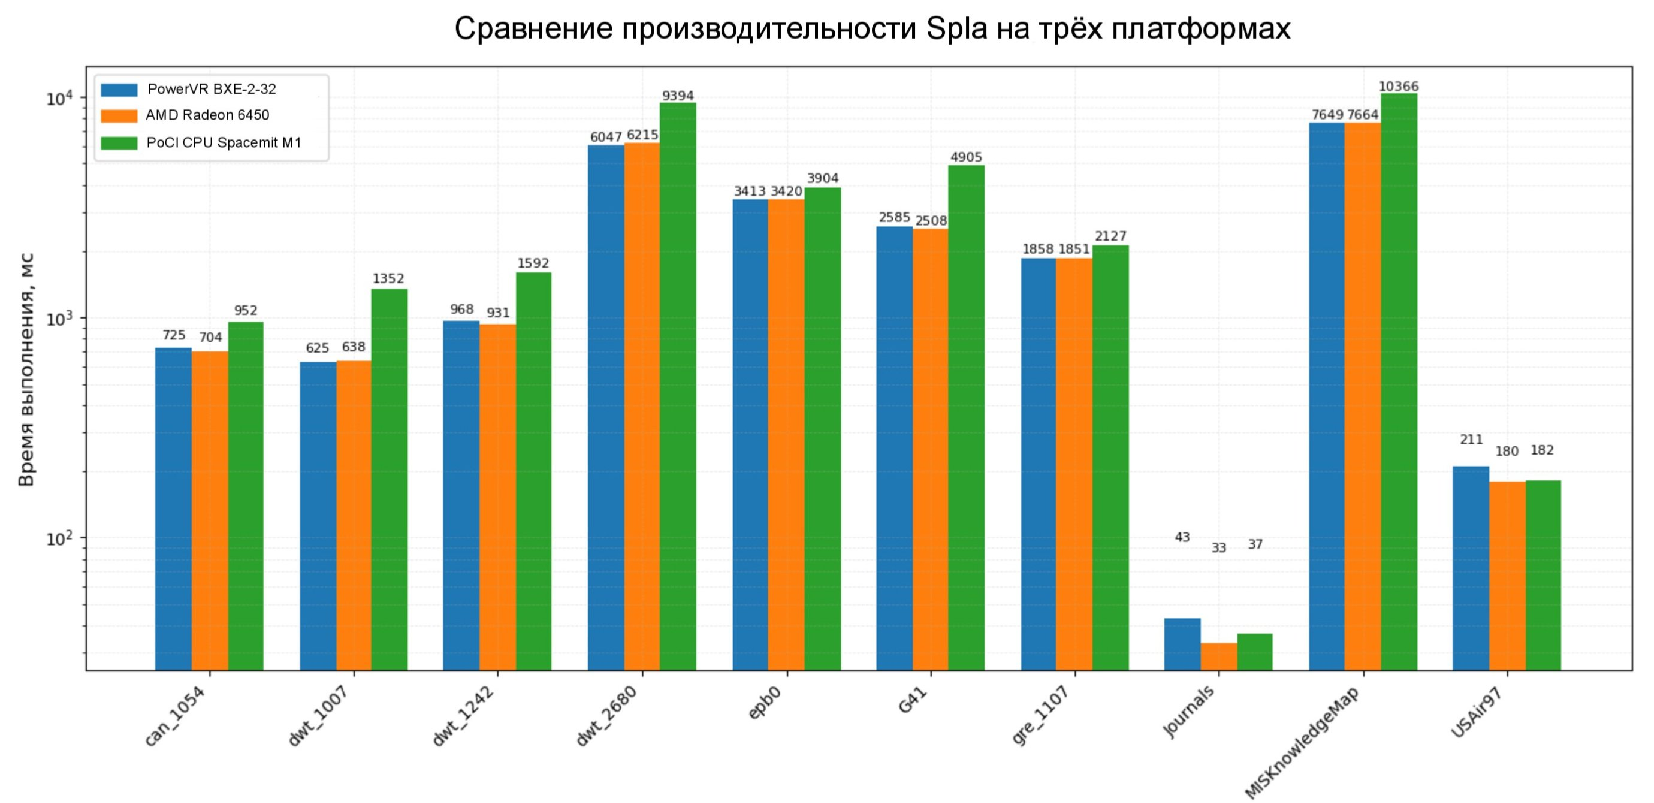
\includegraphics[width=0.909\linewidth]{pictures/milk-v-gpus.pdf}
        \end{center}
\end{frame}

\begin{frame}[fragile]
  \frametitle{RISC-V GPGPU \href{https://github.com/vortexgpgpu/vortex}{Vortex}}
  \begin{itemize}
    \item Набор инструкций, основанный на RISC-V ISA
    \item Поддержка OpenCL через POCL 
    \item Полностью открытая реализация полного стека
    \begin{itemize}
      \item RTL-дизайн (System Verilog)
      \item Компиляторный стек (POCL, LLVM)
      \item Компоненты времени исполнения
      \item Стек разработчика (симуляторы и т.д.)
    \end{itemize}
    \begin{itemize}
      \item[\faGears] Spla должен запускаться
    \end{itemize}
    \item Проблемы со сбросом регистров
    \begin{itemize}
      \item Типичные оптимизации не работают
      \item \href{https://github.com/vortexgpgpu/vortex/issues/251}{Issue 1}
      \item \href{https://github.com/vortexgpgpu/vortex/issues/205}{Issue 2}
    \end{itemize}
    \item В целом, есть подозрение, что мало регистров
    \item Для ПЛИС с HBM
    \begin{itemize}
      \item[\faQuestion] Бонус для обработки слабоструктурированных данных
    \end{itemize}
  \end{itemize}
\end{frame}


\begin{frame}[fragile]
  \frametitle{RISC-V GPGPU \href{https://github.com/THU-DSP-LAB/ventus-gpgpu}{Ventus}}
  \begin{itemize}
    \item Набор инструкций, основанный на RISC-V ISA
    \item Поддержка OpenCL через POCL 
    \item Полностью открытая реализация полного стека
    \begin{itemize}
      \item RTL-дизайн (System Verilog)
      \item Компиляторный стек (POCL, LLVM)
      \item Компоненты времени исполнения
      \item Стек разработчика (симуляторы и т.д.)
    \end{itemize}
    \begin{itemize}
      \item[\faGears] Spla должен запускаться
    \end{itemize}
    \item Проблемы со сбросом регистров
    \begin{itemize}
      \item Типичные оптимизации не работают
      \item \href{https://github.com/vortexgpgpu/vortex/issues/251}{Issue 1}
      \item \href{https://github.com/vortexgpgpu/vortex/issues/205}{Issue 2}
    \end{itemize}
    \item В целом, есть подозрение, что мало регистров
    \item Для ПЛИС с HBM
    \begin{itemize}
      \item[\faQuestion] Бонус для обработки слабоструктурированных данных
    \end{itemize}
  \end{itemize}
\end{frame}







\begin{frame}[fragile]
  \frametitle{Пара слов про \href{https://github.com/vortexgpgpu/vortex}{Vortex}: RISC-V GPGPU}
  \begin{itemize}
    \item Набор инструкций, основанный на RISC-V ISA
    \item Поддержка OpenCL через POCL 
    \begin{itemize}
      \item Spla запускается (и даже что-то работает)
    \end{itemize}
    \pause
    \item Проблемы со сбросом регистров
    \begin{itemize}
      \item Типичные оптимизации не работают
      \item \href{https://github.com/vortexgpgpu/vortex/issues/251}{Issue 1}
      \item \href{https://github.com/vortexgpgpu/vortex/issues/205}{Issue 2}
    \end{itemize}
    \item В целом, есть подозрение, что мало регистров
    \item Проблемы с поддержкой OpenCL
    \begin{itemize}
      \item Атомарные операции 
      \item Некоторые функции работы с буферами (\texttt{clBuffer})
      \item \ldots
    \end{itemize}
    \item Для ПЛИС с HBM
    \begin{itemize}
      \item[\faQuestion] Бонус для обработки граф-структурированных данных
    \end{itemize}
    
  \end{itemize}
\end{frame}

\begin{frame}[fragile]
  \frametitle{Перспективы: RISC-V}
  \begin{itemize}
    \item Идёт работа над расширениями\footnote{Оставим в покое RVV, Integrated Matrix Extension, XuanTie Matrix Extension, \ldots}   
    \begin{itemize}
      \item \href{https://ieeexplore.ieee.org/abstract/document/10546747}{IndexMAC: A Custom RISC-V Vector Instruction to Accelerate Structured-Sparse Matrix Multiplications}, 2024 год
      \item \href{https://dl.acm.org/doi/abs/10.1007/978-3-031-40843-4_35}{Optimizations for Very Long and Sparse Vector Operations on a RISC-V VPU: A Work-in-Progress}, 2023 год
      \item \href{https://dl.acm.org/doi/10.1109/TC.2025.3533083}{Optimizing Structured-Sparse Matrix Multiplication in RISC-V Vector Processors}, 2025 год
      \item \href{https://ieeexplore.ieee.org/abstract/document/10271722}{Sparse Stream Semantic Registers: A Lightweight ISA Extension Accelerating General Sparse Linear Algebra}, 2023 год
      \item \href{https://ieeexplore.ieee.org/abstract/document/11113397}{Hardware/Software Co-Design of RISC-V Extensions for Accelerating Sparse DNNs on FPGAs}, 2024 год       
    \end{itemize}
    \item В основном для машинного обучения: малая разрядность, относительно большая плотность, фиксированный набор типов и операций (часто для инференса)
    \item Vortex: \href{https://cea.hal.science/cea-05043041v1/document}{GPGPUs on FPGAs: A competitive approach for scientific computing?}, 2025 год
  \end{itemize}
\end{frame}

\begin{frame}[fragile]
  \frametitle{Заключение}  
  \begin{itemize}
    \item Высокопроизводительная разреженная линейная алгебра $\Rightarrow$ высокопроизводительные приложения
    \begin{itemize}
      \item Машинное обучение
      \item Графовые базы данных
      \item Анализ социальных, банковских и других сетей
      \item Анализ кода
      \item $\ldots$
    \end{itemize}
    \item Сделать \textbf{разреженную} линейную алгебру высокопроизводительной \textbf{сложно}
    \begin{itemize}
      \item Нерегулярный доступ к данным
      \item Хорошая алгебра --- \textbf{обобщённая} алгебра
      \item Сложности с балансировкой нагрузки
      \item $\ldots$
    \end{itemize}
    \item Есть попытки решить проблему
    \begin{itemize}
      \item Вряд ли на основе RISC-V появится хоть сколько-то универсальное решение\footnote{И дело не в RISC-V}
    \end{itemize} 
  \end{itemize}
\end{frame}

\appendix

\begin{frame}[fragile]
  \frametitle{Семён Григорьев}
  \begin{minipage}{0.70\textwidth}
  \begin{itemize}    
    \item Доцент кафедры системного программирования Санкт-Петербургского Государственного Университета
    \item Научный сотрудник лаборатории YADRO
    \item Руководитель исследовательской группы
    \item Области интересов
    \begin{itemize}
      \item \textbf{Высокопроизводительная линейная алгебра} для анализа графов
      \begin{itemize}
        \item \textbf{Обобщённая}: матрицы и вектора параметризованы типом элемента, операции над ними могут быть заданы пользователем
        \item \textbf{Разреженная}: специализированные структуры для хранения матриц и векторов, специализированные алгоритмы для их обработки 
        \item В том числе, с использованием \textbf{графических ускорителей}
      \end{itemize}
      \item \textbf{Высокопроизводительный анализ графов}      
    \end{itemize}
    \end{itemize}
\end{minipage}
\begin{minipage}[t]{0.29\textwidth}
  \begin{center}
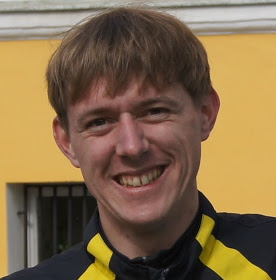
\includegraphics[width=0.8\textwidth]{pictures/SemyonGrigorev.jpg}
  \end{center}
  {\scriptsize
\begin{itemize}    
  \item Email: s.v.grigoriev@mail.spbu.ru
  \item GitHub: \href{https://github.com/gsvgit}{gsvgit}
  \item Google Scholar: \href{https://scholar.google.com/citations?hl=ru&user=kP4dqUAAAAAJ&view_op=list_works&sortby=pubdate}{Semyon Grigorev}
  \item DBLP: \href{https://dblp.org/pid/181/9903.html}{Semyon V. Grigorev}
\end{itemize}
  }
\end{minipage}
\end{frame}

\end{document}
